Aufgrund des Umfangs der Blocklib und der Unübersichtlichkeit an einigen Stellen kann das Jobsystem nicht, wie in Abbildung~\vref{fig:optimalArchitecture} gezeigt, umfassend integriert werden. Um die Anforderungen von Kapitel~\ref{sec:anforderungen} zu erfüllen, wird daher ein Jobsystem implementiert, das nur an ausgewählten Stellen mit der Blocklib konsolidiert wird und ansonsten für die zukünftige Nutzung bereitsteht.


\begin{figure}
	\centering
	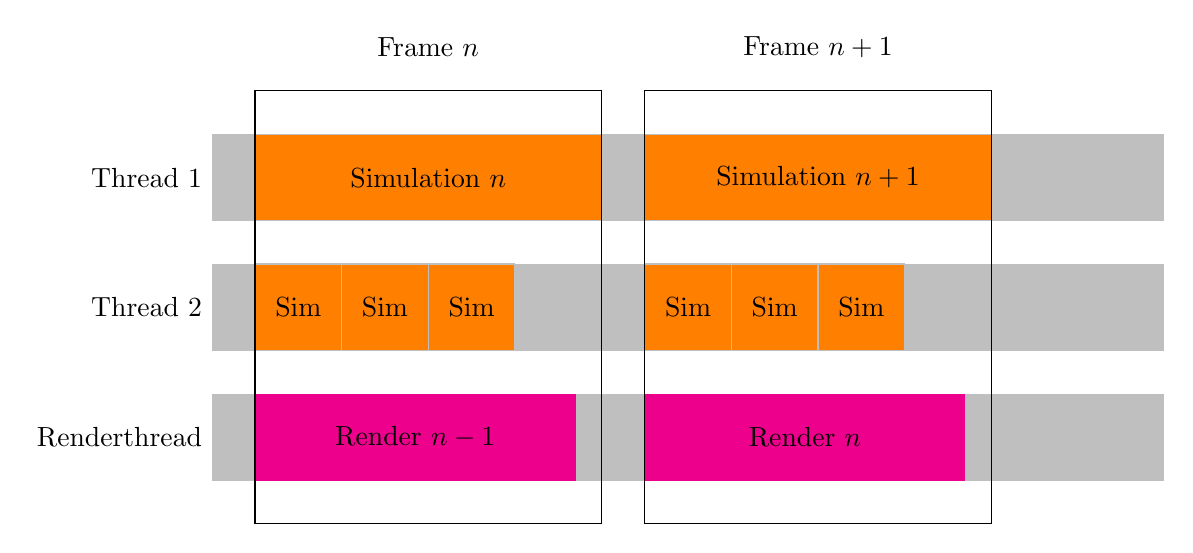
\begin{tikzpicture}[scale=1.1]
		\fill[lightgray]  (0,0) rectangle (11,1);
		\fill[lightgray] (0,-1.5) rectangle (11,-0.5);
		\fill[lightgray]  (0,1.5) rectangle (11,2.5);
		
		\node[anchor=east] at (0,2) {Thread 1};
		\node[anchor=east] at (0,0.5) {Thread 2};
		\node[anchor=east] at (0,-1) {Renderthread};
		
		
		\fill [orange,draw=lightgray] (0.5,1.5) rectangle node[black] {Simulation $n$} (4.5,2.5);
		\fill [orange,draw=lightgray] (0.5,0) rectangle node[black] {Sim} (1.5,1);
		\fill [orange,draw=lightgray] (1.5,0) rectangle node[black] {Sim} (2.5,1);
		\fill [orange,draw=lightgray] (2.5,0) rectangle node[black] {Sim} (3.5,1);
	
		\fill [orange,draw=lightgray] (5,1.5) rectangle node[black] {Simulation $n+1$} (9,2.5);
		\fill [orange,draw=lightgray] (5,0) rectangle node[black] {Sim} (6,1);
		\fill [orange,draw=lightgray] (6,0) rectangle node[black] {Sim} (7,1);
		\fill [orange,draw=lightgray] (7,0) rectangle node[black] {Sim} (8,1);
	
		\fill [magenta] (0.5,-0.5) rectangle node[black]{Render $n-1$} (4.2,-1.5);
		\fill [magenta] (5,-0.5) rectangle node[black]{Render $n$} (8.7,-1.5);
		
		\node at (2.5,3.5) {Frame $n$};
		\node at (7,3.5) {Frame $n+1$};
		
		\draw  (0.5,3) rectangle (4.5,-2);
		\draw  (5,3) rectangle (9,-2);
	\end{tikzpicture}
	\caption[Design der neuen Multithreading-Architektur der Blocklib.]{Design der neuen Multithreading-Architektur der Blocklib. Statt einer Simulation, die vollständig aus Jobs besteht, gibt es einen langen Simulations-Job, der aber weitere Jobs starten kann. \enquote{Sim} kennzeichnet einen Simulationsjob.}\label{fig:plannedArchitecture}
\end{figure}


Da das Jobsystem keine vollständige Integration in die Blocklib erfährt, verändert sich die Architektur konzeptuell leicht. Diese Änderung ist in Abbildung~\vref{fig:plannedArchitecture} zu sehen. Anstatt die gesamte Simulation in viele kleine Jobs zu zerlegen, bleibt eine sequentialisierte Simulation bestehen, die dann aber die Möglichkeit besitzt, weitere nebenläufige Jobs zu starten. Mit dieser Architektur ist es möglich, die Blocklib inkrementell zu der in Abbildung~\vref{fig:optimalArchitecture} gezeigten Architektur umzuwandeln, indem in zukünftigen Arbeiten immer mehr pseudo-sequentialisierte \glspl{Anweisung} der Simulation als nebenläufige Jobs definiert werden, bis sie vollständig aus Jobs besteht.

Java bietet mit dem Interface \class{ExecutorService} bereits eine gute und bekannte Schnittstellendefinition, die für ein Jobsystem genutzt werden kann. Daher baut das Design des Jobsystems der Blocklib auf diesem Interface auf. 

\begin{figure}
	\includesvg[width=\textwidth]{GrobesDesign.svg}
	\caption[Struktur des entwickelten Jobsystems.]{Struktur des entwickelten Jobsystems. Das in der Blocklib definierte Interface wird von dem Interface \class{ScheduledExecutorService} abgeleitet. Damit steht ein für Java-Entwickler bekanntes Interface bereit, das erweitert wird.}\label{fig:GrobesDesign}
\end{figure}

In Abbildung~\vref{fig:GrobesDesign} ist die Struktur des Designs für das Jobsystem der Blocklib dargestellt. Es wird ein Interface \class{BlocklibExecutorService} definiert, das von dem Interface \class{ScheduledExecutorService} der Java Bibliothek abgeleitet ist. Das Interface wird so erweitert, dass die verschiedenen \code{submit(...)} Methoden jeweils Objekte des Typs \class{CompletableFuture} zurückgeben. Die \code{schedule(...)} Methoden geben jeweils ein \class{ScheduledCompletableFuture} Objekt zurück, das später noch näher erläutert wird.

Das Interface \class{BlocklibExecutorService} wird durch die Klasse \class{BlocklibExecutor} implementiert. Sie nutzt zur Durchführung von Jobs den von der Java Bibliothek definierten \class{ScheduledThreadPoolExecutor}. Um die für die Rückgabewerte nötigen \class{CompletableFuture} Objekte zu erzeugen, wird eine Klasse \class{CompletableFutureWrapper} erstellt. Eine vollständige Auflistung der von den drei Interfaces bereitgestellten Methoden ist in Anhang~\vref{appendix:BlocklibExecutorService} zu finden. 

Die API des Jobsystems bietet verschiedene Methoden, um nebenläufige \glspl{Anweisung} zu starten. Mittels der \code{submit(...)} Methoden können \glspl{Anweisung} definiert werden, die so bald wie möglich ausgeführt werden. Da diese Methoden ein \class{CompletableFuture} Objekt zurückgeben, lassen sich über die dort definierten Methoden einfach nachgelagerten nebenläufige \glspl{Anweisung} definieren, die abhängig von der Vollendung der ursprünglichen \gls{Anweisung} ausgeführt werden. Mit den \code{schedule(...)} Methoden wird analog dazu eine Möglichkeit geboten \glspl{Anweisung} zu definieren, die nach Ablauf eines bestimmten Zeitintervalls nebenläufig ausgeführt werden. Mittels \code{scheduleAtFixedRate(...)} und \code{scheduleWithFixedDelay(...)} können periodisch durchzuführende \glspl{Anweisung} zur Ausführung gebracht werden.